\documentclass[12pt,a4paper]{article}
%\usepackage{xcolor} \pagecolor[rgb]{0.5,0.5,0.5} \color[rgb]{1,1,1}
%\usepackage[utf8]{inputenc}
\usepackage[shortlabels]{enumitem}
%\usepackage{bm}
\usepackage{mathrsfs}
\usepackage{amsmath}
\usepackage{amssymb}
\usepackage{hyperref}
\usepackage{graphicx}
\begin{document}
\title{Solutions to BDA Assignment 1,
 2020/2021 Semester 2}
\author{Theodoros Ladas, s2124289}
\date{\today}
\maketitle

\vspace{1cm}

\noindent\textbf{1)}
\begin{enumerate}[(a)]
%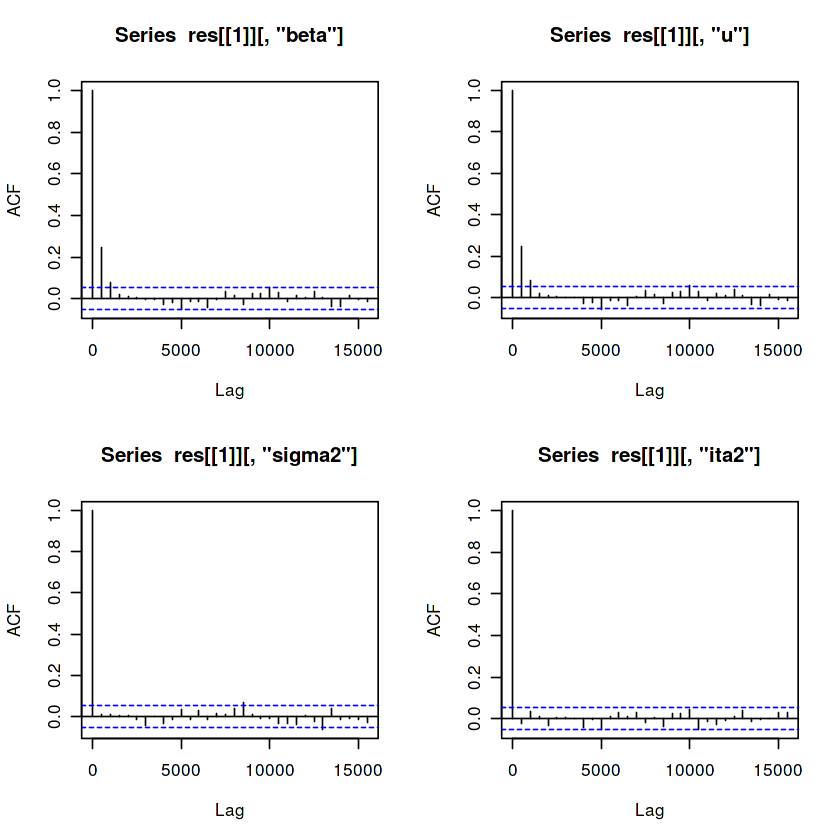
\includegraphics[scale=0.3]{./images/1_Figure0.png}
\item

Explanation: A state-space model is built in this assignment in order to model the population (log-population) of whales, with data from 1952 up to 1997. The model is divided into the state model 
$x_t = b x_{t-1}+u+w_t; \quad w_t\sim N(0,\sigma^2)$, and an observation model $y_t =x_{t}+v_t, \quad v_t\sim N(0,\eta^2)$. Here the meaning of the parameters of the model will be discussed, specifically, $b, u, \sigma^2, \eta^2$. 

The $b$ parameter, is the coefficient that connects the previous log-population, to the current one. In other words, if there is no noise on our data, therefore the relationship being completely deterministic, the log-population of the whales would change from $t=i$ to $t=i+1$ by $b$. 

The $u$ parameter, is the intersect of the state model, and its interpretation is: $u$ would be the log-population of whales at time $t=0$.

The $\sigma^2$ parameter, is the parameter of the variance of random noise of the underlying state model discribed above. 

Finally, the $\eta^2$ parameter, has a similar explanation to the $\sigma^2$ parameter as it also is the parameter of variance of random noise, but this time it represents the noise of the observation equation. That means that even if our underlying model was deterministic, there is also an extra uncertainty in our model, because of the observation error that might occur.

The point of modeling the log-population of whales with this state-space model, is that now, we can have priors on all this parameters, that are going to be updated from our dataset in later stages. 

\item
Explanation: The dataset had some missing values that needed to be addressed before continuing with building the engine of the model. First of all the missing data came in two different ways, first of all, there where years in the dataset where the popuplation observed was reported as NA, and secondly there where missing years from the data, indicating that the observed population for that year, is NA. On the first group, no additional imputation step was taken, because the model was going to be evaluated using JAGS (Just Another Gibbs Sampler). JAGS, treats these kinds of NAs as stochastic nodes, meaning that they are another part of our model. On the other had, the second kind of NAs, was treated by injecting into the dataset the years that where completely missing allong with an NA for the observed population value.

The priors for the model are stated here. It was assumed that $x_0 \sim N(\text{log}(2500),1)$, $b \sim U(0,1)$, $u \sim \text{exp}(1)$ and finaly, $\sigma^2, \eta^2 ~ \text{inv-Gamma}(0.1,0.1)$

The burn in period for which the data are discarded for computing estimated of these parameters, was selected to be $2,000$ iterations, and the whole simulation run for $700,000$ iterations.

\item
Explanation: In order to check the mixing of the chains, the Gelman-Rubin statistic was calculated. The Diagrams below, show this statistic per iteration. One idicates that there is no evidence that show a problem of the mixing of the chains. We can see that on iteration $700,000$ the statistic is either at one, of very close to it ($1.01$) for all the parameters of the model, so this is a good sign. Also, a second way that the mixing of the chains was evaluated, was by the autocorrealtion plots. These are shown below as well per parameter. What we can observe is that for the first iteration the autocorrelation is $1$, which is expected since we are using a Markov-Chain model. However, either on the second lag, or very quicly after that the autocorrelation of the point explored by the algorithm, versus the previous one, goes to $0$ and stays there. That is also a very good indication that the algorithm is not 'stuck' on a small space of the parameter space and instead explores the whole space. 

Results:

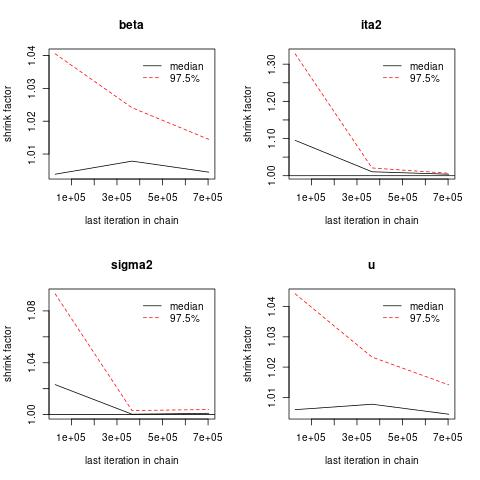
\includegraphics[scale=0.44]{./images/1_Figure00_gelman.jpg}
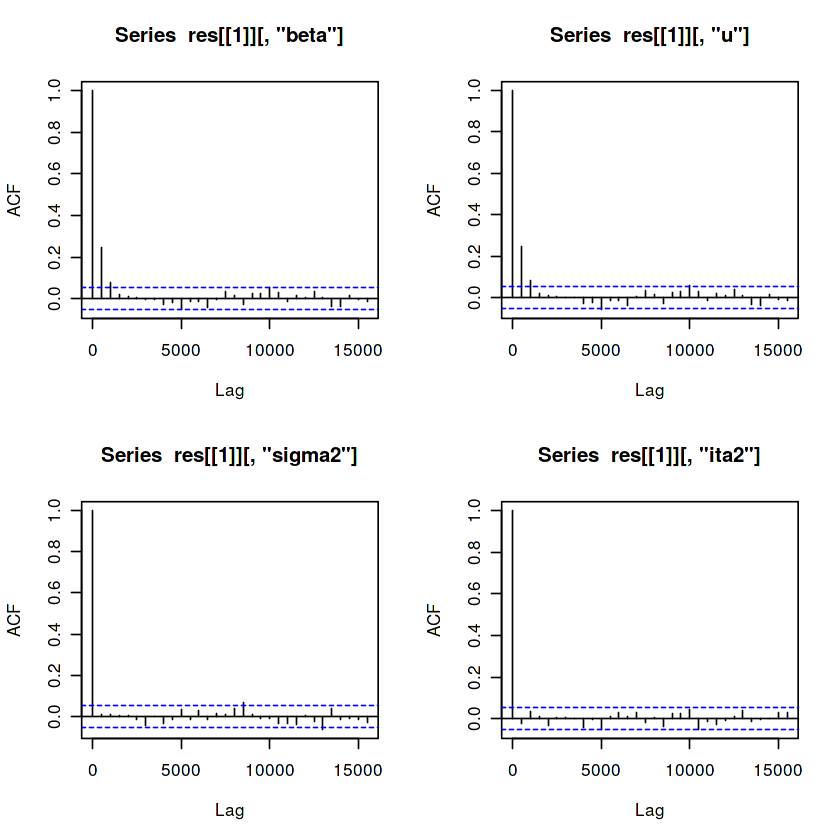
\includegraphics[scale=0.25]{./images/1_Figure0.png}

\item
Explanation: Here the results from the above simulation are presented. 

\includegraphics[scale=0.25]{./images/1_Table0.png}

We can see that the mean and standard deviation values for all the parameters, as well as confidence intervals for each parameter.

Below the plot of the posterior densities and their prior densities are also plotted. From these diagrams we can clearly see that the prior is not dominating the posterior in any case, so our choice of prior densities and hyperparameters is reasonable. In order to further robustify the method, later a sensitivity analysis, will be performed.

Results:

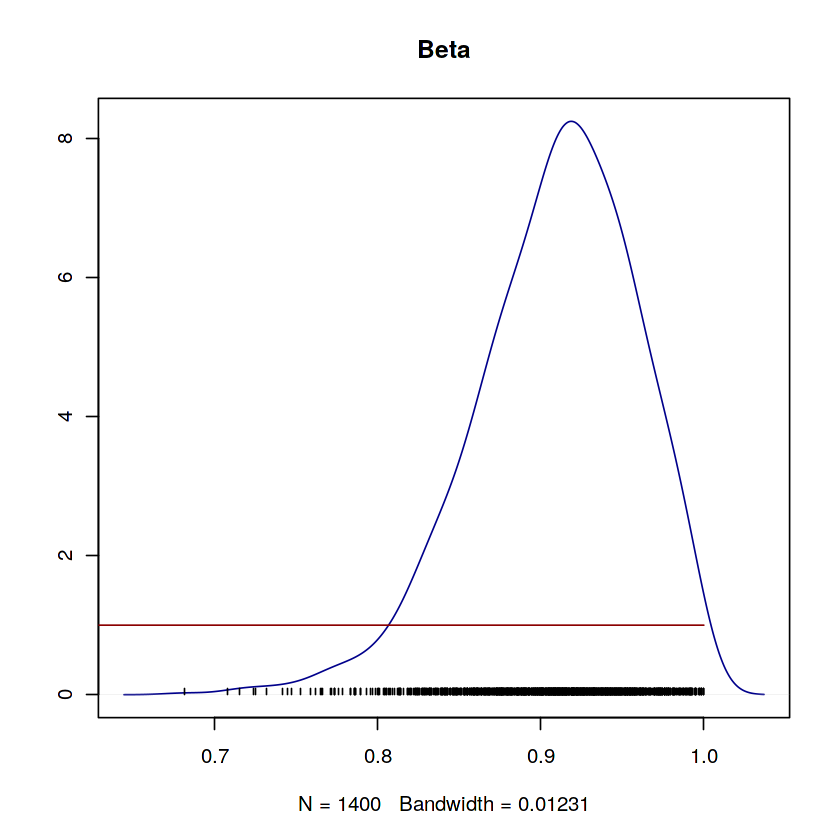
\includegraphics[scale=0.25]{./images/1_Figure3_beta_posterior.png}
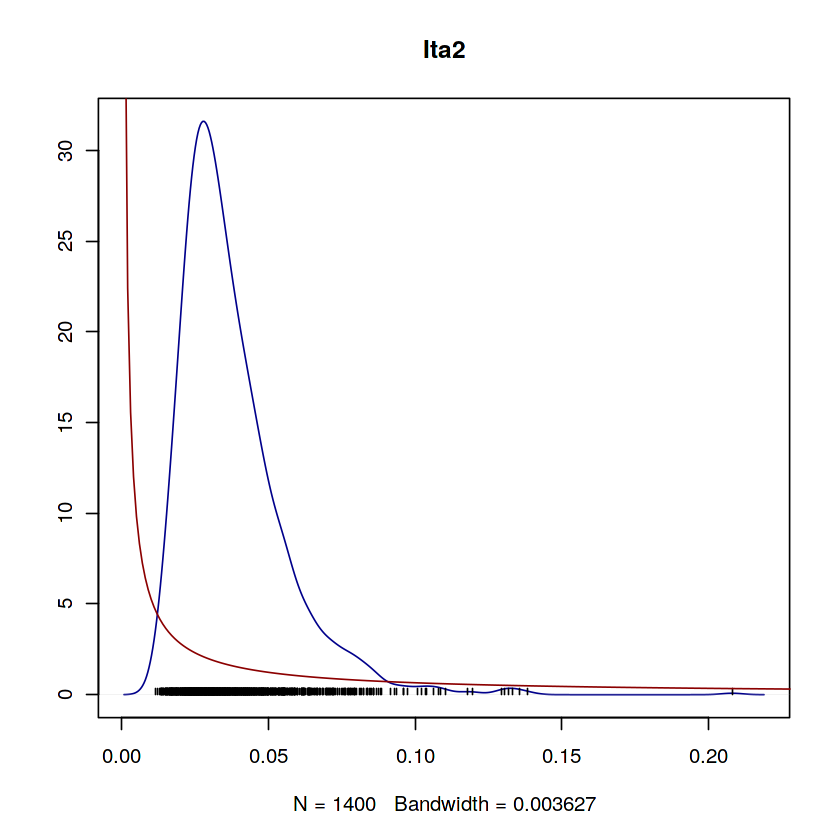
\includegraphics[scale=0.25]{./images/1_Figure3_ita_posterior.png}


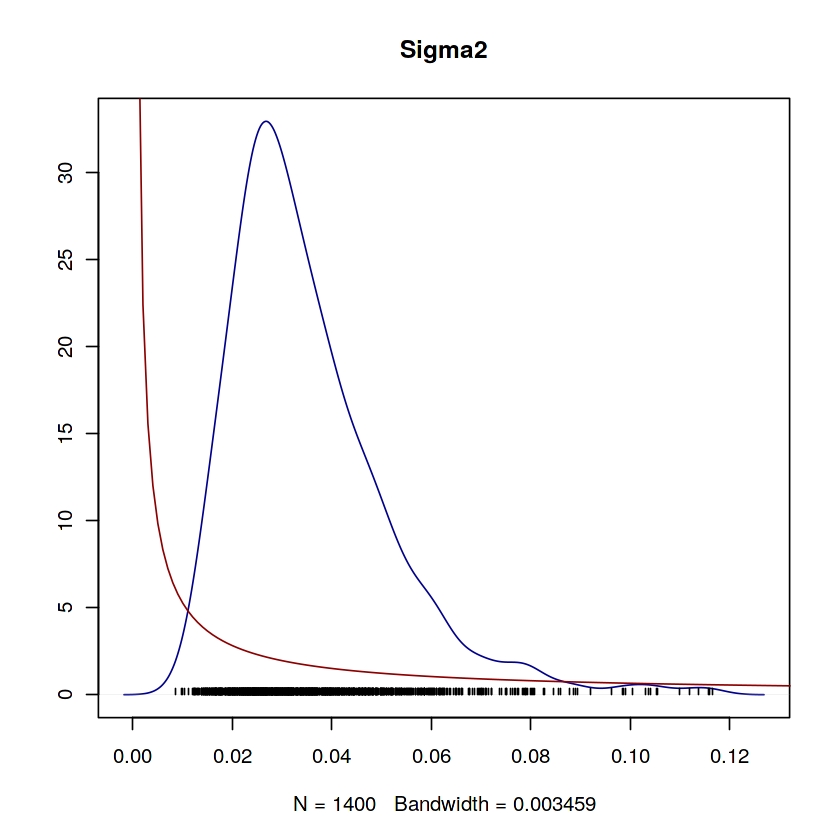
\includegraphics[scale=0.25]{./images/1_Figure3_sigma_posterior.png}
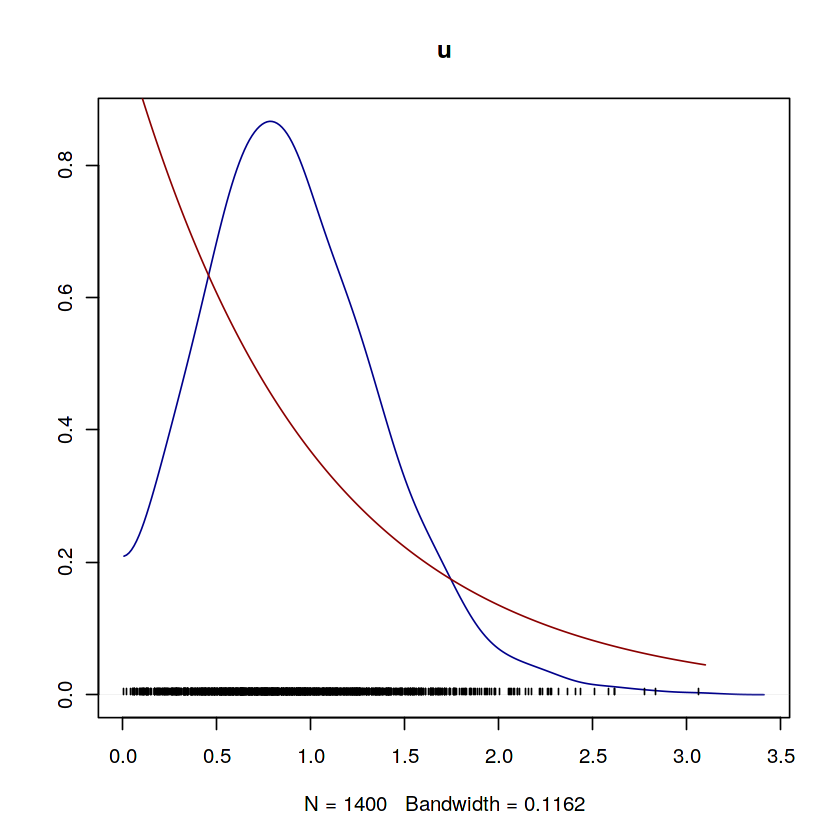
\includegraphics[scale=0.25]{./images/1_Figure3_u_posterior.png}

\item
Explanation: Here the sensitivity analysis is discussed. The priors where chosen as follows. The distribution for the prior of each parameter stayed the same and the choice of starting hyperpareters was vastly different, in order to see whether the results will change or not.
More specifically, $b \sim U(-1,2)$, $u \sim \text{exp}(3)$ and finaly, $\sigma^2, \eta^2 ~ \text{inv-Gamma}(1/0.1,1/0.1)$. The prior for $x_0$ stayed the same. 

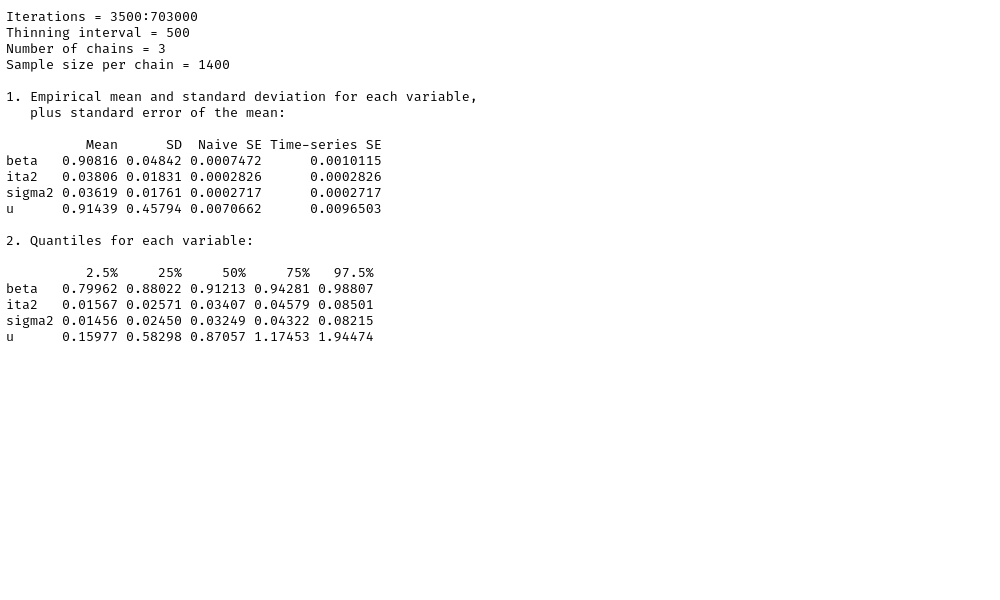
\includegraphics[scale=0.25]{./images/1_table1.png}

As we can see the results changed to the fourth significant digit. This clearly idicated that the prior doesn't dominate the posterior and it makes it even more likely that the posterior density is converging to the true value of the parameters. The autocorellation plot figure for this model is also present in the results graph, used as in the first model to check the mixing of the new chains.

Results:

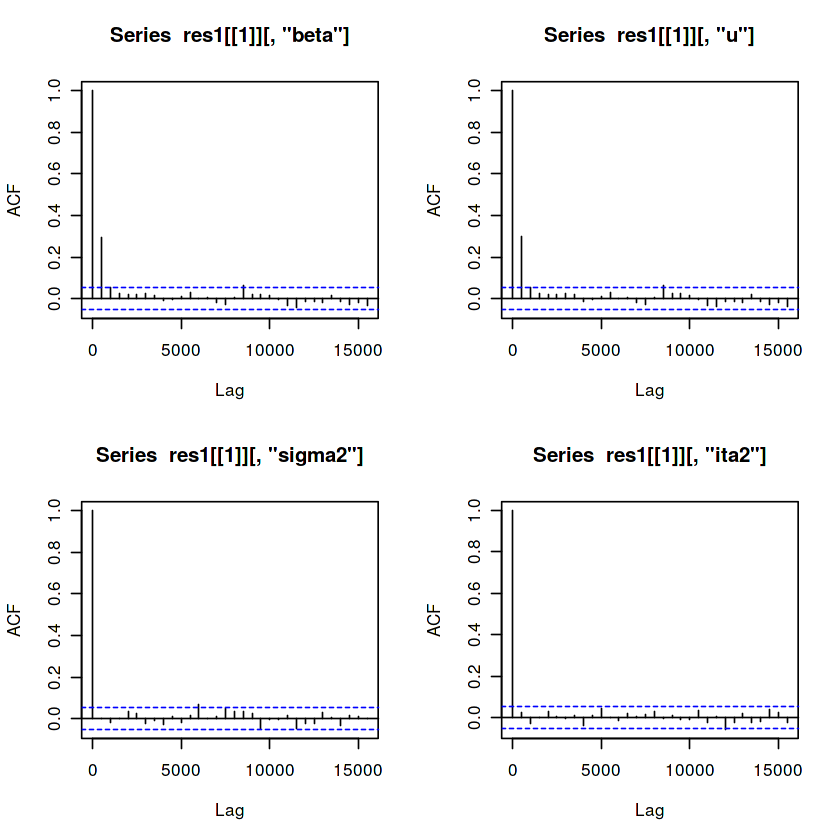
\includegraphics[scale=0.30]{./images/1_Figure4_acf.png}

\item
Explanation: On the below graph, the evolution of the posterior mean of log-population of whales is presented. This line is projected to 2050. The dotted lines show the 95\% Confidence intervals (the lower line is the 2.5\% and the upper line the 97.5\%). We see that the mean get's stable after a while, which is what we expected since the $\beta$ coefficient was around $0.9$. A $\beta$ of $1$ idicates a stationary process in the AR(1) model. We also see the 95\% CI for the mean to diverge very heavily. This is because our last observed datapoint is in 1997 and we are trying to predict 2050. This divergence explained because the state-model has a random noise and the observed values model has another small random noise. All these 'mistakes' add up, making the projection for 2050 have a very big variance associated with it.
Also the posterior probability that the population of gray whales becores smaller than 100 at any year from 1951 until the end of 2050 was calculated to be 0. Or mathematically, $p(\min_{t\in \{0,1\ldots,99\}} x_t<=\log(100)|y) = 0$

Results:

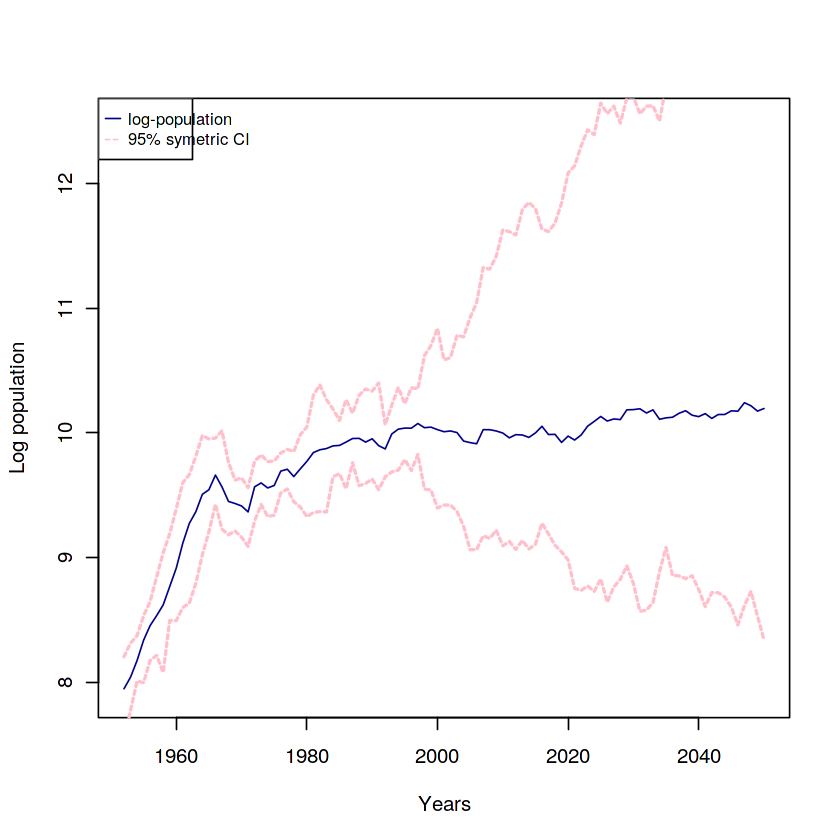
\includegraphics[scale=0.25]{./images/1_Figure5_final_plot.png}


\item
Explanation: Finally, posterior predictive checks for various statistics, specifically, the min, the max and the mean, to evaluate the fit of this model, where the prior are the original ones stated in section (b) was performed. The results are reported below in the form of histograms of the posterior predictive samples generated from the model. The red lines indicate the min, the max and the mean of the given sample that we observed respectively. We can clearly see that in all cases the line is well within the bounds of the histograms. The most extreme case is that of the min, but even this is still acceptable as it is within $2 \sigma$ from the mean of its distribution.

Results:

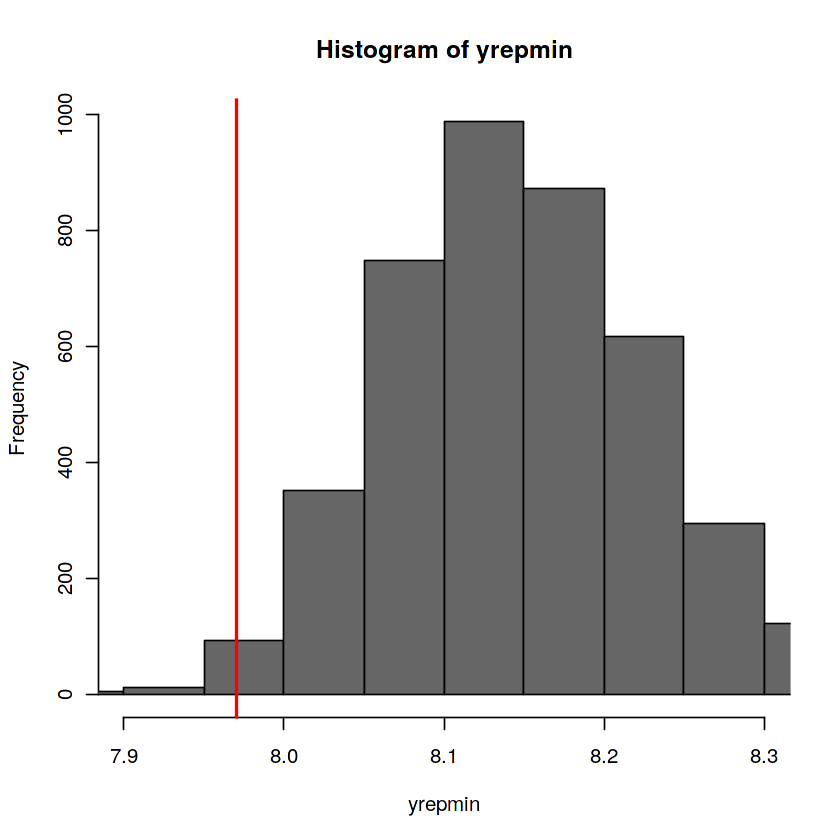
\includegraphics[scale=0.17]{./images/1_Figure6_predictive_0.png}
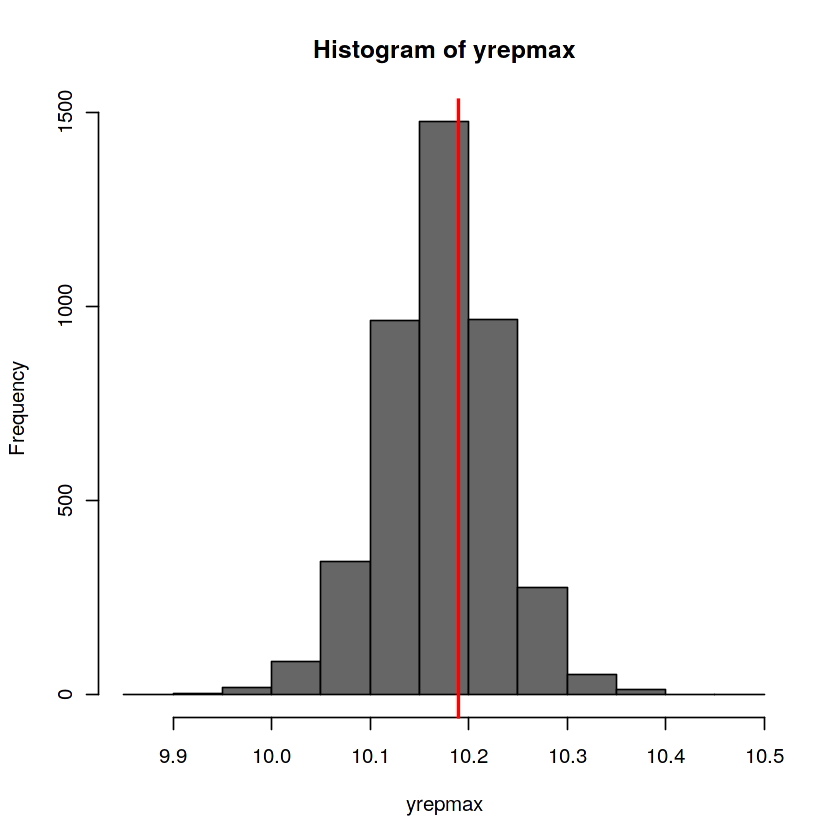
\includegraphics[scale=0.17]{./images/1_Figure6_predictive_1.png}
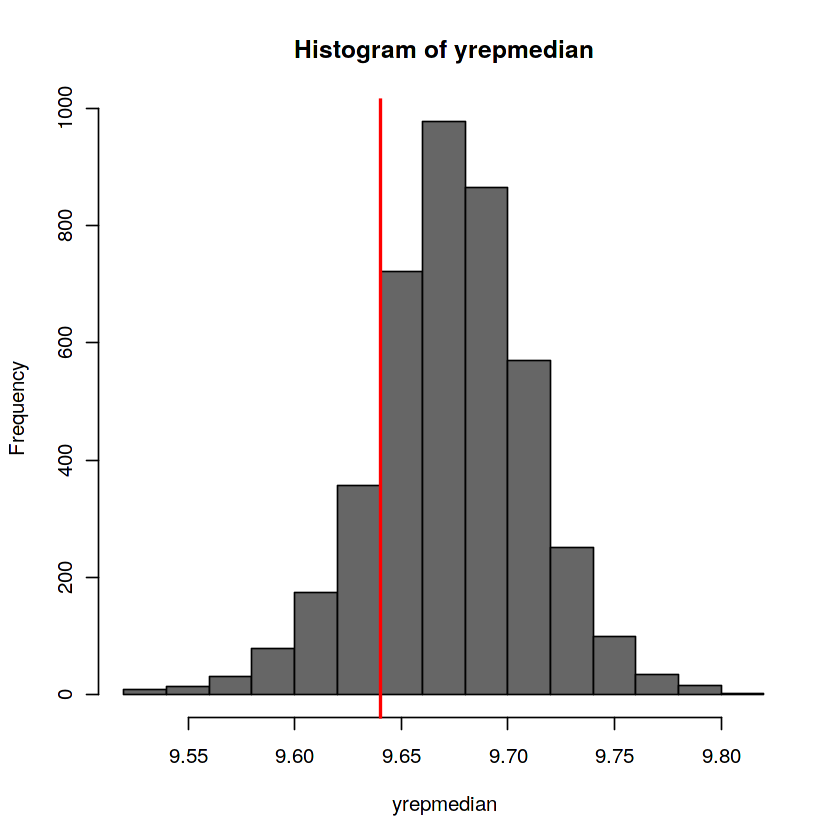
\includegraphics[scale=0.17]{./images/1_Figure6_predictive_2.png}



\end{enumerate}

\noindent\textbf{2)}
\begin{enumerate}[(a)]
\item
Explanation: In this problem, the aim is to model house prices per unit area from recent transactions in Taipei. Our dataset consists of 414 rows of 6 features (house age, distance from nearest MRT (metro) station in meters, number of convenience stores within walking distance, latidude, longitude and the target of the price). First of all, the data matrix was centered. That means that for every feature, its mean has been subtracted in order to shift their distribution to have a zero mean, and then each value have been divided by their standard deviation in order to make every feature to have a unit variance. Then since we will again work on the log scale, the target variable of the price has been converted to log-price. Then a standard linear regression was fit, with the defaults \textsf{lm} function of \textsf{R}. This was done to have a benchmark. Later, more complicated models can be fit and their quality of fit can be compared to the standard linear regression. 

Results:

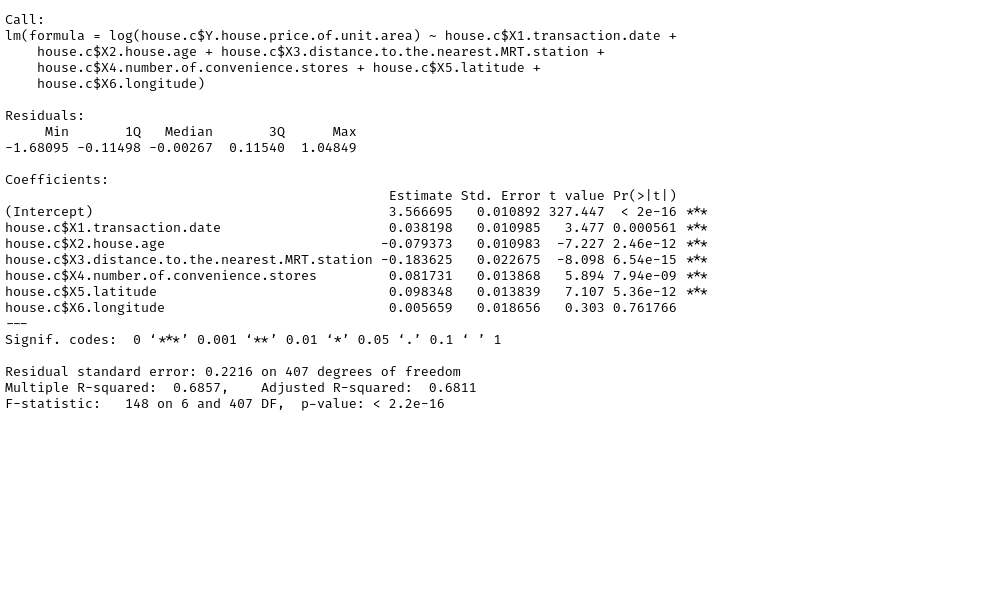
\includegraphics[scale=0.28]{./images/2_table0.png}


\item
Explanation: For the purposes of this problem, an Integrated Nested Laplace Approximation (INLA) model was choosen. The posterior of the model, was a $\text{Gamma}(0.1,0.1)$ and the Gaussian prior with mena zero and variance $1e6$ was choosen in order to represent prior ignorance of the value of the parameters of the model. The mean standard error of the fit was $4.47$. More summary statistics are presented in the Results section. This model, immidiately had a very positive effect in the standard deviation of the mean residuals of the model, since it is $0.22$. The negative sum log of the conditional predictive ordinate (NSLCPO) was also produced and it is $-28.78$. 

Finally, a plot of the posterior density for the variance parameter $\sigma^2$ is also shown below. The figure shows that the variance parameter $\sigma^2$ has a mean value of around $0.05$ with a very high confidence, since we can see that most of the density on the diagram is on the interval $\{0.04, 0.06\}$. So we are fairly sure that a small, non-zero variance exist in the noise parameter of the model.

Results:

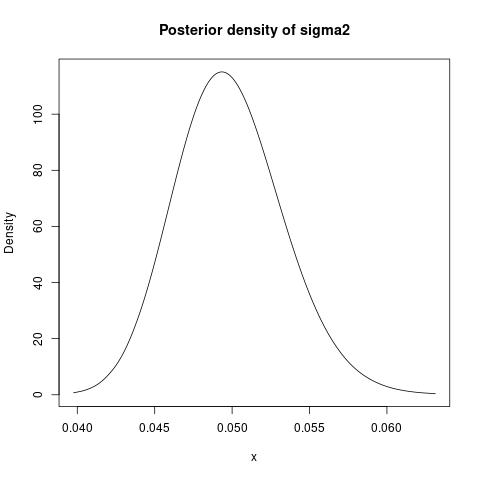
\includegraphics[scale=0.5]{./images/post.jpg}



\item
Explanation: Next we evaluate the fit of the model, by producing multiple plots for the residuals of the fit. On the first diagram we see the normal quantile-quantile plot for the Bayesian studentized residuals of the fit. In red we see the line of 45 degrees. We can observe that almost all the residuals fall onto this line, and that means that the distribution of the residuals is not far from a Normal distribution. So our error term has a Normal distribution and our assumption of homoskedasticity holds. On the next diagrams we see the Bayesian studentized residuals against the fitted values. This plot was done in order to check if any patterns are aparent. That would indicate that there is some correlation between the residuals and the fitted values which is another important assumption of our linear model. It is clear that no apparent pattern emerges from this diagram so we can continue with our analysis.

Results:

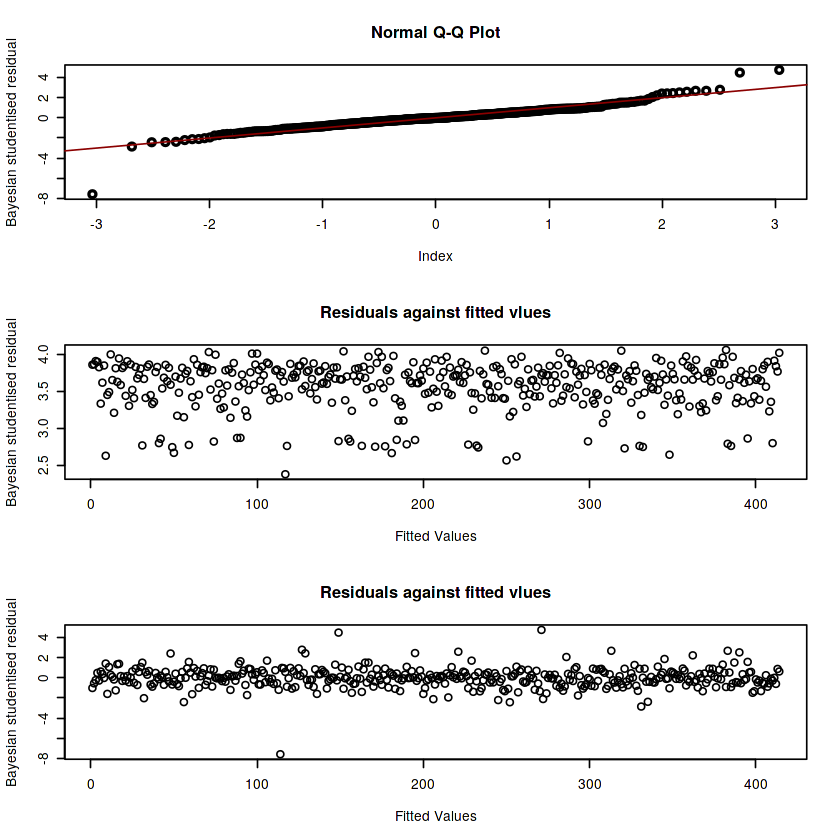
\includegraphics[scale=0.5]{./images/2_Figure1_qq.png}


\item
Explanation: Next, a robust to outliers version of the model was considered. This has exactly the same priors as the original model discribed in (b). The NSLCPO score of the model was $-77.9$, which is lower than the first model, indicating a better fit. The corresponding DIC value was $-157.09$ and the standard deviation of the mean residuals was $0.222$ which also indicated a better fit. On the results section there are two posterior density graphs, one for the degrees of freedom and another of $\sigma^2$ as before. We can clearly see that the mean value for the degrees of freedom is around $3$, which indicated that there are some outliers skew the Student-t distribution. Lastly, we see a small increase of the mean variance. This is expected, as we are not using the information of some data points due to the robust regression. 
The summary statistic is also included below. 

Results:

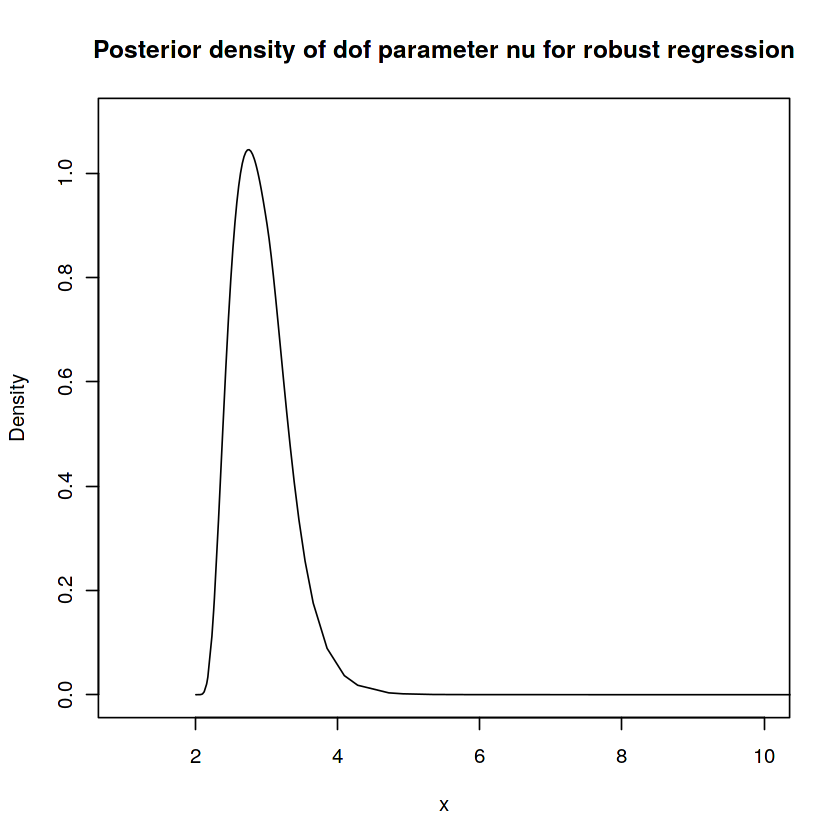
\includegraphics[scale=0.25]{./images/2_Figure2_df.png}
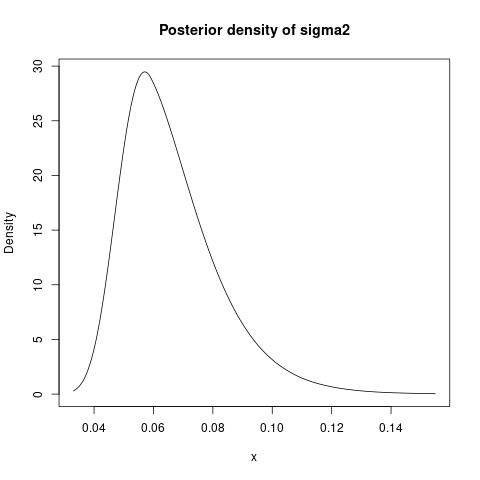
\includegraphics[scale=0.440]{./images/posterior.jpg}

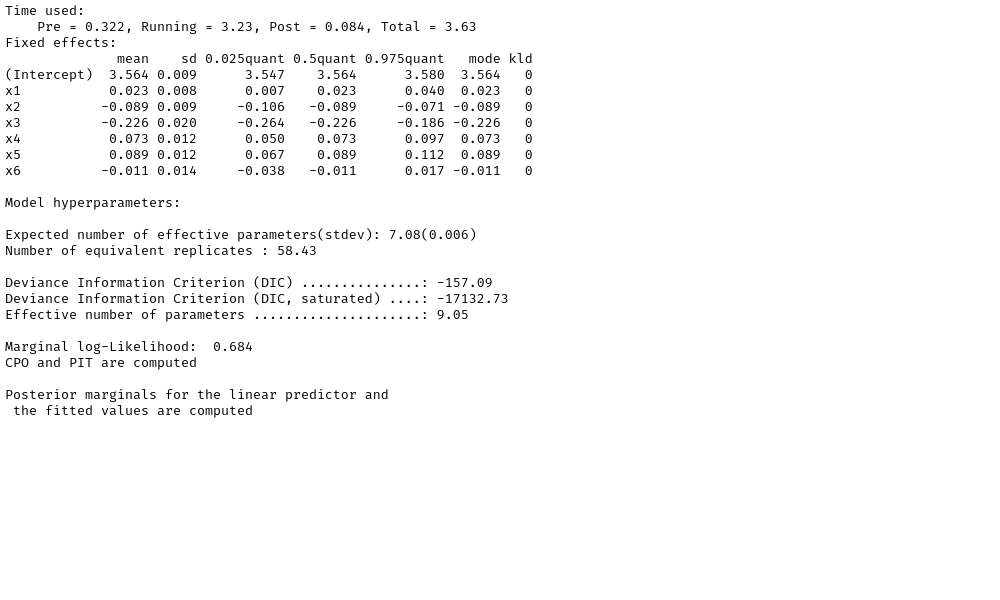
\includegraphics[scale=0.440]{./images/2_table3.png}
d
\item
Explanation: The next step was to consider our variable $x_4$ (number of convenience stores within walking distance) as a categorical variable with multiple factors. We then fitted the two models (simple and robust) with the new modified variable in order to check whether this change will affect the model in a positive way. 

NSLCPO simple: $-28.02$ 

NSLCPO robust: $-84.45$

MSE simple: $0.2155$

MSE robust: $0.2172$

It is clear from the NSLCPO score, that the best model so far, is the one with $x_4$ as a categorical variable and with robust regression as this produces the lowest overal NSLCPO score.
Lastly, the Mean standard deviation of the mean residuals of both models is lower than the previous one. The non-robust model seems to have a bit lower MSE, but this is obvious only on the third significant digit. 

Below you can find summary statistics for both models.

Results:

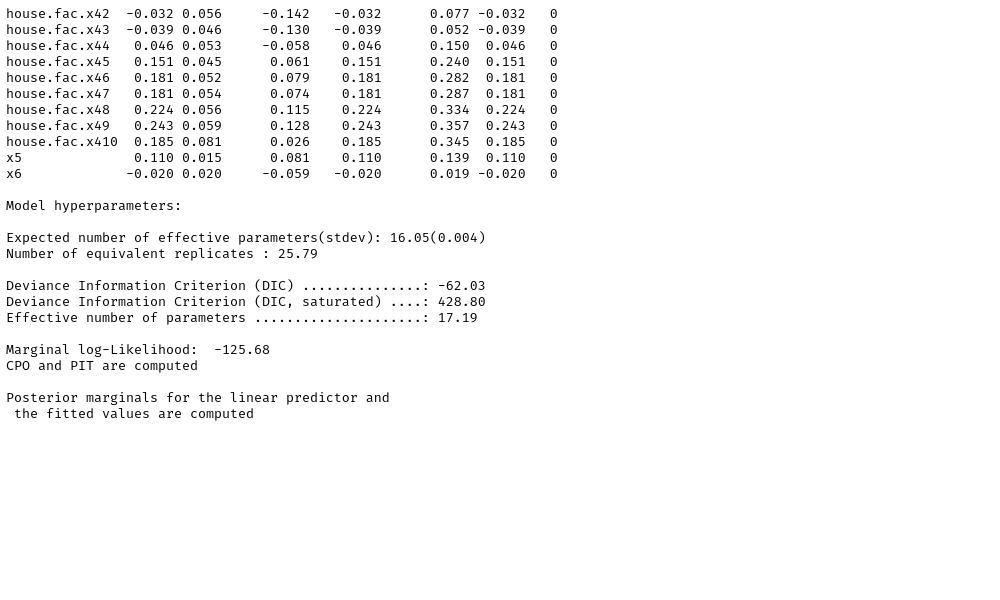
\includegraphics[scale=0.440]{./images/2_table4.png}
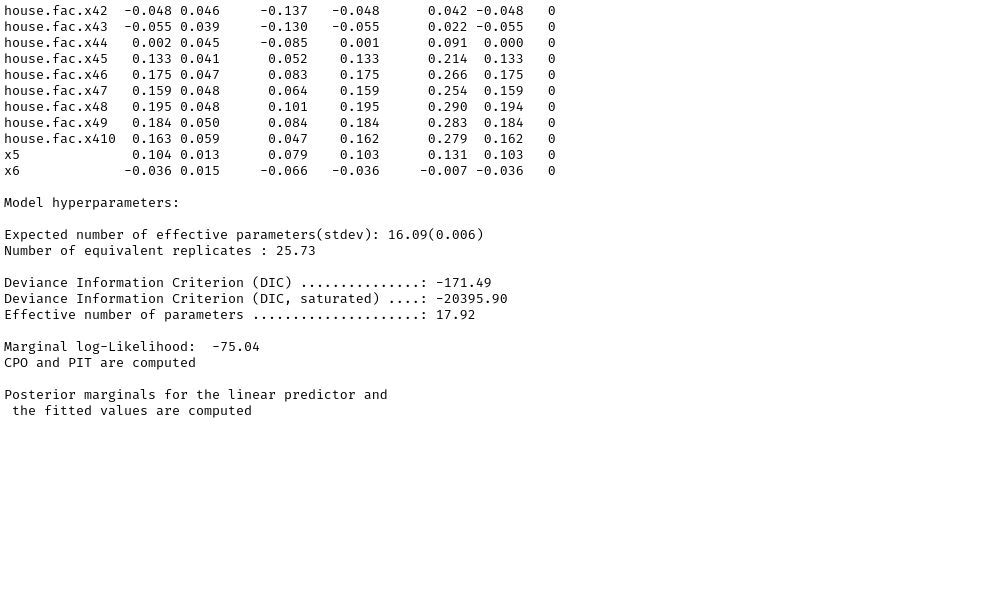
\includegraphics[scale=0.440]{./images/2_table5.png}


\item
Explanation: Lastly a non linear in feature model was considered to explore the possibility of non-linear relationship in the data. The model that we considered is the following: 

$\hat{y} = \hat{\beta_0} + \hat{\beta_1}x_1 + ... + \hat{\beta_6}x_6 + \hat{\beta_7}x_1^2 + \hat{\beta_8}x_2^2 + \hat{\beta_8}x_3^2 + \hat{\beta_9}x_5^2 + \hat{\beta_{10}}x_6^2$

Essentially taking into consideration a relationship of second degree. 

NSLCPO transformed: $-112.82$

DIC transformed: $-231.32$

MSE transformed: $0.203$

The NSLCPO score shows a significant improvent over all other models, which is also apparent on the MSE score of the model. Summary statistics are presented below. At this point a very important caveat needs to be mentioned. Up until now we are only considering in sample \it{goodness of fit} measures. That means that there is a chance that we have overfitted our model to our observed data. In order to check that we could compute all the above quantinties on a held-out set, or even perform a k-fold cross validation. This is left for further development of the model.

Results:

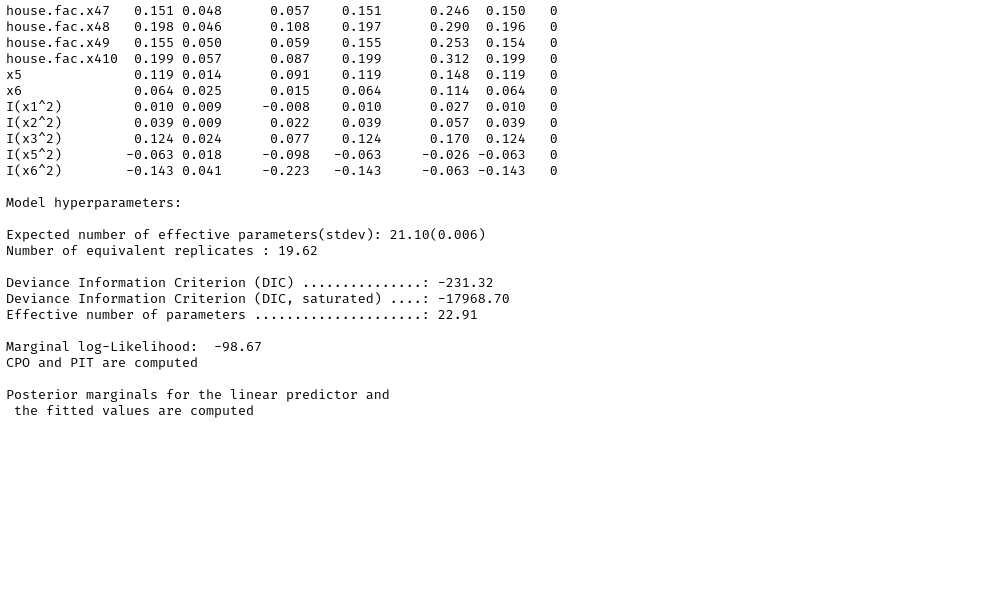
\includegraphics[scale=0.440]{./images/2_table6.png}

\item
Explanation: Finally, using our original model from part (b), we will predict the prices for the three next years



Results:

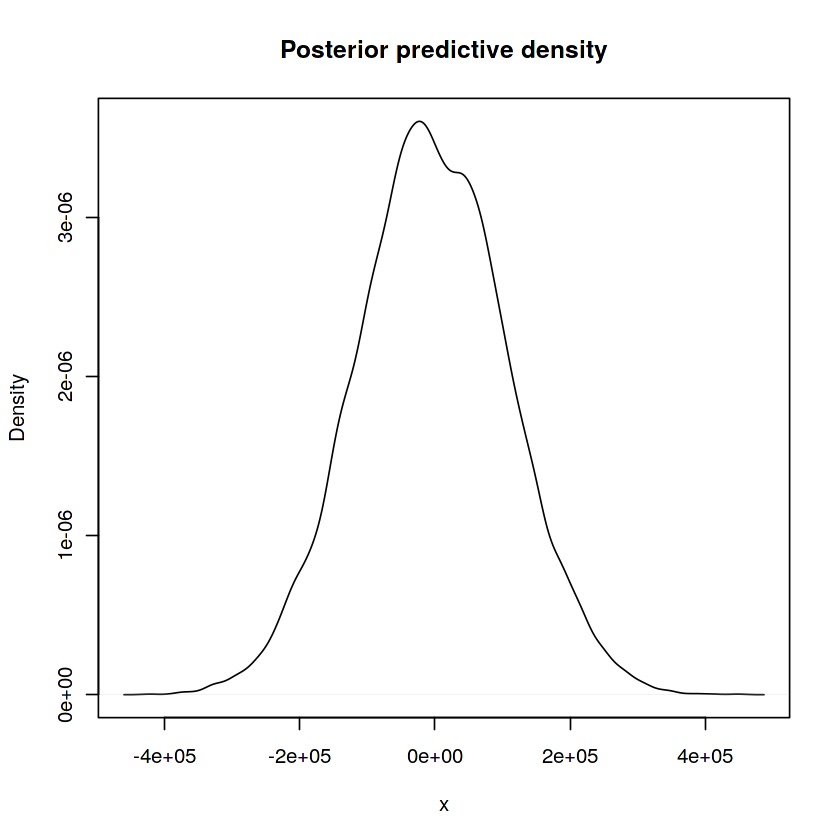
\includegraphics[scale=0.440]{./images/2_Figure3_final.png}


\end{enumerate}
\end{document}